\documentclass[VM.tex]{subfiles}

\begin{document}

\subsubsection*{Description : }
Simply Supported Circular plate with point load at the center.  
\subsubsection*{Reference : }
S.Timoshenko , S . Woinowsky , Theory of Plates and Shells , pg:69, Article : 19 . 
\subsubsection*{Material and Geometric data : }


\begin{figure}[h!]
\centering
\subfile{TIM69_DRAW.tex}
\caption{TIM69}% \label{TIM69sch}
\end{figure}
\begin{table}[ht]
\renewcommand{\arraystretch}{1.5}
\centering
\caption{Input Data}
%\label{my-labelsdqf}
\begin{tabular}{|ll|ll|ll|}
\hline
\multicolumn{2}{|l|}{\cellcolor[HTML]{C0C0C0}Material Property} & \multicolumn{2}{l|}{\cellcolor[HTML]{C0C0C0}Geometric Data} & \multicolumn{2}{l|}{\cellcolor[HTML]{C0C0C0}Loading Data} \\ \hline  \hline
Young's Modulus ($E$)          & 5E11 $Pa$         & Radius ($r$)        & 1 $m$        & Point Load ($F_z$)        & -1000 $N$         \\
Poission's Ratio ($\nu$)       & 0.3         &  Thickness($t$)     &         0.01 $m$  &         &  \\ 
            \hline
\end{tabular}
\end{table}




\subsubsection*{Mesh and boundary condition : }





\begin{figure}[h!]
\begin{subfigure}{.45\textwidth}
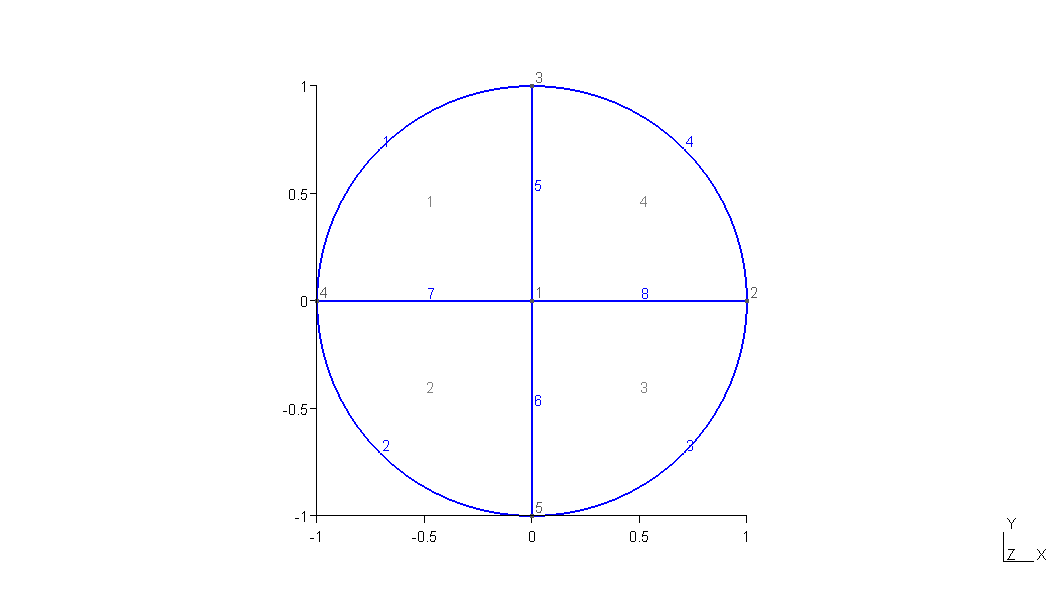
\includegraphics[width=\linewidth,trim={8cm 0 8cm 0},clip]{TIM68/TIM68_geo.png}
%\caption{Mode Shape 4}
\end{subfigure} \hfill
\begin{subfigure}{.45\textwidth}
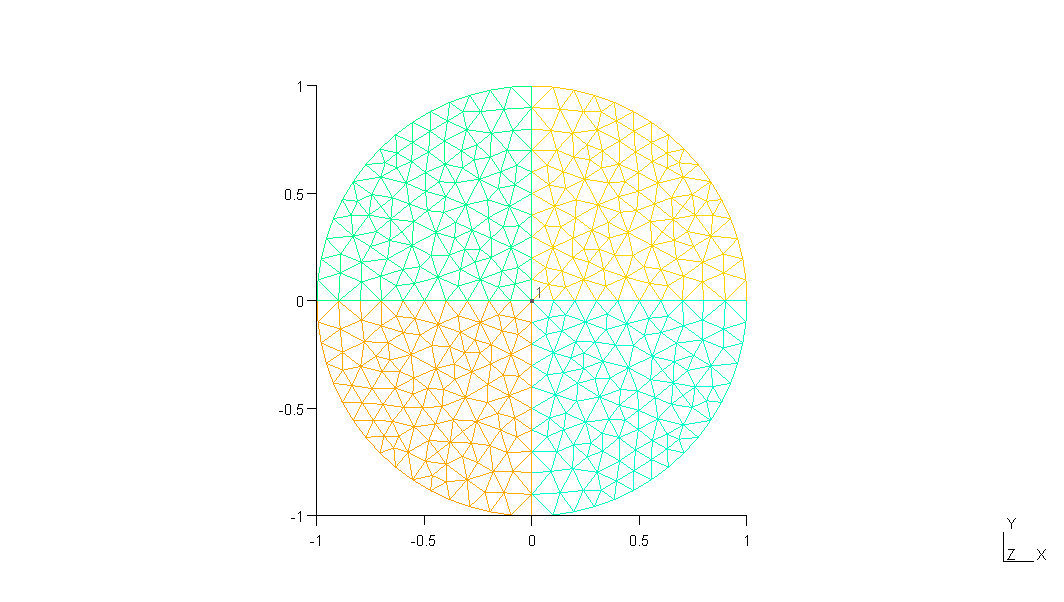
\includegraphics[width=\linewidth,trim={8cm 0 8cm 0},clip]{TIM68/TIM68_msh.png}
%\caption{Mode Shape 5}
\end{subfigure}
\caption{Geomentry and Mesh of TIM68}
\end{figure}





\begin{table}[h!]
\renewcommand{\arraystretch}{1.5}
\centering
\caption{FEM and Boundary condition data}
%\label{my-label}
\begin{tabular}{|l|lll|l|lll|}
\hline
 \multicolumn{4}{l|}{\cellcolor[HTML]{C0C0C0}Direchlet Boundary} & \multicolumn{4}{l|}{\cellcolor[HTML]{C0C0C0}Neumann Boundary} \\ \hline \hline
  Geo - \newline Entity      & $w$          & $\theta _ x$     & $\theta _ y $    & Geo - \newline Entity         & $F_z$        & $M_x$        & $M_y$        \\ \hline    
 line \{1,2,3,4\}                   & Fixed      & Fixed         & Fixed        & Point \{1\}                    & -1000 $N$        &           &           \\ \hline
\end{tabular}
\end{table}
\subsubsection*{Analytically solution : }
The target analytically solution given as
\begin{equation}
w = \frac{F_z}{16 \pi D}\left[ r^2 - a^2 \right]+\frac{F_zr^2}{8 \pi D}\left[ log \frac{a}{r} \right]
\end{equation} 
The displacement at center is obtained by substituting $a\approx0$. The analytical solution is -0.000434 $m$.

\subsubsection*{Result and error analysis : }

\begin{figure}[h!]
\centering
\minipage{0.8\textwidth}%
  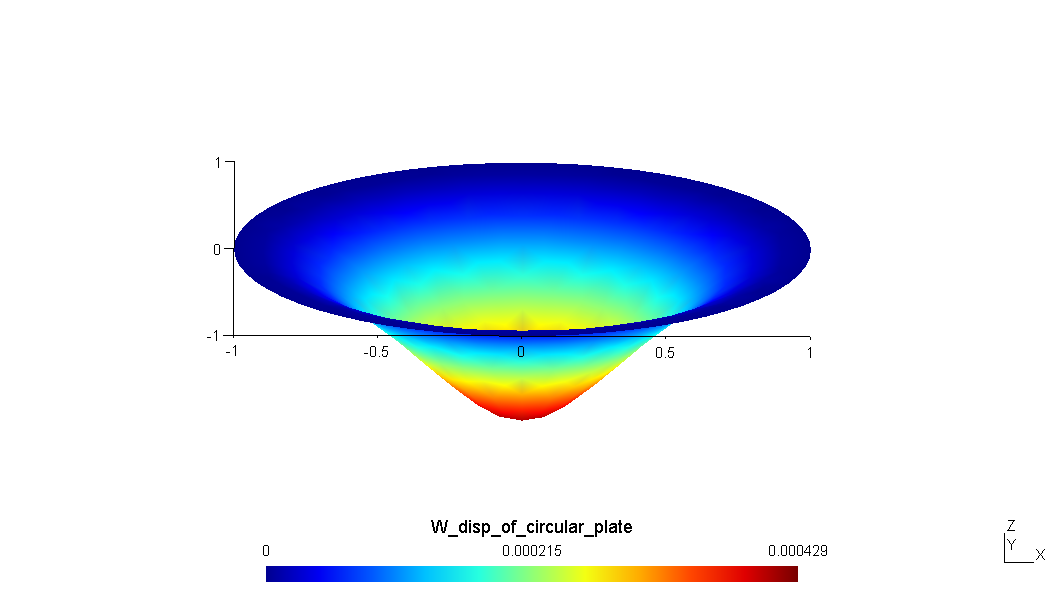
\includegraphics[width=\linewidth,trim={0 0 0 5cm},clip]{TIM69/TIM69_pos.png}
  \caption{FEM solution plot}
\endminipage
\end{figure}
The maximum displacement of the domain is our solution . w displacement at center is $ -0.000429 in $.


So the Error percentage is $ 1.26 \% $. 

\end{document}